
%%%%%%%%%%%%%%%%%%%%%%% file typeinst.tex %%%%%%%%%%%%%%%%%%%%%%%%%
%
% This is the LaTeX source for the instructions to authors using
% the LaTeX document class 'llncs.cls' for contributions to
% the Lecture Notes in Computer Sciences series.
% http://www.springer.com/lncs       Springer Heidelberg 2006/05/04
%
% It may be used as a template for your own input - copy it
% to a new file with a new name and use it as the basis
% for your article.
%
% NB: the document class 'llncs' has its own and detailed documentation, see
% ftp://ftp.springer.de/data/pubftp/pub/tex/latex/llncs/latex2e/llncsdoc.pdf
%
%%%%%%%%%%%%%%%%%%%%%%%%%%%%%%%%%%%%%%%%%%%%%%%%%%%%%%%%%%%%%%%%%%%


\documentclass[runningheads,a4paper]{llncs}

\usepackage{amssymb}
\setcounter{tocdepth}{3}
\usepackage{graphicx}
%\usepackage{listings}

\usepackage{url}
\urldef{\mailsa}\path|{alfred.hofmann, ursula.barth, ingrid.haas, frank.holzwarth,|
\urldef{\mailsb}\path|anna.kramer, leonie.kunz, christine.reiss, nicole.sator,|
\urldef{\mailsc}\path|erika.siebert-cole, peter.strasser, lncs}@springer.com|    
\newcommand{\keywords}[1]{\par\addvspace\baselineskip
\noindent\keywordname\enspace\ignorespaces#1}

\begin{document}

\mainmatter  % start of an individual contribution

% first the title is needed
\title{Semantic Annotation Semantically: Using a~Shareable Extraction Ontology and a Reasoner}

% a short form should be given in case it is too long for the running head
\titlerunning{Semantic Annotation Semantically}

% the name(s) of the author(s) follow(s) next
%
% NB: Chinese authors should write their first names(s) in front of
% their surnames. This ensures that the names appear correctly in
% the running heads and the author index.
%
\author{Jan D\v{e}dek \and Peter Vojt\'{a}\v{s}}
%\thanks{Please note that the LNCS Editorial assumes that all authors have used
%the western naming convention, with given names preceding surnames. This determines
%the structure of the names in the running heads and the author index.}%
%
\authorrunning{Jan D\v{e}dek \and Peter Vojt\'{a}\v{s}}
% (feature abused for this document to repeat the title also on left hand pages)

% the affiliations are given next; don't give your e-mail address
% unless you accept that it will be published
\institute{Department of Software Engineering, Charles University,\\
Prague, Czech Republic
\\\url{{dedek,vojtas}@ksi.mff.cuni.cz}}

%
% NB: a more complex sample for affiliations and the mapping to the
% corresponding authors can be found in the file "llncs.dem"
% (search for the string "\mainmatter" where a contribution starts).
% "llncs.dem" accompanies the document class "llncs.cls".
%

%\toctitle{Semantic Annotation Semantically: Using a Shareable Extraction Ontology and a Reasoner}
%\tocauthor{Jan D\v{e}dek and Peter Vojt\'{a}\v{s}}
\maketitle


\begin{abstract}
In this paper we present a method for semantic annotation of texts, which is based on a deep linguistic analysis (DLA) and Inductive Logic Programming xxxxxxxxxxxxxxxxxxxxxxxx

A description, implementation and initial evaluation of the method are the main contributions of the paper.
\keywords{Semantic Annotation, Dependency Linguistics, Inductive Logic Programming, Information Extraction, Machine Learning}
\end{abstract}


\section{Introduction}

Dedek ISWC:
\cite{biblio:DedekISWC2010}

\begin{figure}
\centerline{\includegraphics[width=\hsize]{img/semantic_rules_app_schema}}
\caption{Semantic annotation driven by an extraction ontology and a reasoner -- schema of the process.}
\label{img:rules_app_schema}
\end{figure}


\cite{so17864}:
\begin{quote}
An ontology is a formal specification of a shared conceptualization.	
\end{quote}


\cite{Studer1998161}:
\begin{quote}
An ontology is a formal, explicit specification of a shared conceptualization.
\end{quote}


\section{Related Work}
\subsection{Servey}
\cite{citeulike:7291004}
\subsection{Embley}
2004: \cite{Embley:2004:TSU:1012294.1012295} 
2002: \cite{DBLP:conf/er/EmbleyTL02} 
\subsection{Labsk\'{y}}
\cite{springerlink:10.1007/978-3-642-01891-6_5}


\section{Experiment}
\subsection{Linguistics}

PDT: \cite{dedek:PDT20_CD}

TectoMT: \cite{dedek:ZaPtTectoMTHighly2008}



\begin{figure}
\centerline{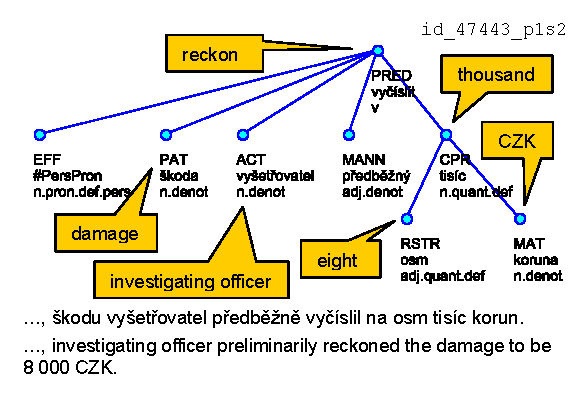
\includegraphics[width=0.5\hsize]{img/tree}}
\caption{Tectogrammatical tree of the sentence: ``Hutton is offering 35 dlrs cash per share for 83 pct of the shares.''}
\label{img:tree}
\end{figure}





\subsection{Data}

We use data contained in the ``Corporate Acquisition Events'' corpus
described in \cite{lewis1992representation}. More precisely we use the \emph{Acquisitions v1.1} version\footnote{This version of the corpus comes form the Dot.kom (Designing infOrmation extracTion for KnOwledge Management) project's resources: \url{http://nlp.shef.ac.uk/dot.kom/resources.html}} of the corpus.
This is a collection of 600 news articles describing acquisition
events taken from the Reuters dataset. News articles are tagged to identify fields
related to acquisition events. These fields include `purchaser' , `acquired', and
`seller' companies along with their abbreviated names (`purchabr', `acqabr' and
`sellerabr') Some news articles also mention the field `deal amount'. Together,
these seven fields define the set of target elements for information extraction
task: we will refer to these fields as �roles� in the rest of the document.

\subsection{Success of such rules}
\cite{DBLP:conf/ilp/RamakrishnanJBS07}

\subsection{Examples of rules}

\begin{figure}
\small
[Rule 1] [Pos cover = 23 Neg cover = 6]\\
\verb@mention_root(acquired,A) :-@\\
\verb@   'lex.rf'(B,A), t_lemma(B,'Inc'), tDependency(C,B), tDependency(C,D),@\\
\verb@   formeme(D,'n:in+X'), tDependency(E,C).@
\smallskip\newline
[Rule 11] [Pos cover = 25 Neg cover = 6]\\
\verb@mention_root(acquired,A) :-@\\
\verb@   'lex.rf'(B,A), t_lemma(B,'Inc'), tDependency(C,B), formeme(C,'n:obj'), @\\
\verb@   tDependency(C,D), functor(D,'APP').@
\smallskip\newline
[Rule 75] [Pos cover = 14 Neg cover = 1]\\
\verb@mention_root(acquired,A) :-@\\
\verb@   'lex.rf'(B,A), t_lemma(B,'Inc'), functor(B,'APP'), tDependency(C,B), @\\
\verb@   number(C,pl).@
	\caption{Examples of extraction rules in the native Prolog format.}
	\label{fig:rules_prolog}
\end{figure}


\begin{figure}
\small
[Rule 1]\\
\verb@lex.rf(?b, ?a), t_lemma(?b, "Inc"), tDependency(?c, ?b),@\\
\verb@tDependency(?c, ?d), formeme(?d, "n:in+X"), tDependency(?c, ?e)@\\
\verb@      -> mention_root(?a, "acquired")@
\smallskip\newline
[Rule 11]\\
\verb@lex.rf(?b, ?a), t_lemma(?b, "Inc"), tDependency(?c, ?b),@\\
\verb@formeme(?c, "n:obj"), tDependency(?c, ?d), functor(?d, "APP")@\\
\verb@      -> mention_root(?a, "acquired")@   
\smallskip\newline
[Rule 75]\\
\verb@lex.rf(?b, ?a), t_lemma(?b, "Inc"), functor(?b, "APP"),@\\
\verb@tDependency(?c, ?b), number(?c, "pl")@\\
\verb@      -> mention_root(?a, "acquired")@   
	\caption{Examples of extraction rules in Prot\'{e}g\'{e} 4 -- Rules View's format}
	\label{fig:rules_protege}
\end{figure}

\begin{figure}
\centerline{\includegraphics[width=0.87\hsize]{img/rules_owl_xml}}
\caption{Rule 75 in the OWL/XML syntax for Rules in OWL 2 \cite{GHPP09a}.}
\label{img:rules_xml}
\end{figure}

\begin{figure}
\small
\begin{verbatim}
@prefix pml: <http://ufal.mff.cuni.cz/pdt/pml/>.
[rule-75:  
        ( ?b pml:lex.rf ?a )
        ( ?c pml:tDependency ?b )
        ( ?b pml:functor 'APP' )
        ( ?c pml:number 'pl' )
        ( ?b pml:t_lemma 'Inc' )
     -> 
        ( ?a pml:mention_root 'acquired' )
]
\end{verbatim}

\caption{Rule 75 in the Jena rules syntax.}
\label{img:rules_jena}
\end{figure}



%\lstinputlisting[language=XML]{img/rule.owl.xml}



%[Rule 1] [Pos cover = 23 Neg cover = 6] 17
%mention_root(acquired,A) :-
%   'lex.rf'(B,A), t_lemma(B,'Inc'), tDependency(C,B), tDependency(C,D), 
%   formeme(D,'n:in+X'), tDependency(E,C).
%
%lex.rf(?b, ?a), t_lemma(?b, "Inc"), tDependency(?c, ?b), tDependency(?c, ?d), formeme(?d, "n:in+X"), tDependency(?c, ?e) -> mention_root(?a, "acquired")   
%
%
%[Rule 11] [Pos cover = 25 Neg cover = 6] 19
%mention_root(acquired,A) :-
%   'lex.rf'(B,A), t_lemma(B,'Inc'), tDependency(C,B), formeme(C,'n:obj'), 
%   tDependency(C,D), functor(D,'APP').
%   
%lex.rf(?b, ?a), t_lemma(?b, "Inc"), tDependency(?c, ?b), formeme(?c, "n:obj"), tDependency(?c, ?d), functor(?d, "APP") -> mention_root(?a, "acquired")   
%
%
%[Rule 75] [Pos cover = 14 Neg cover = 1]   13
%mention_root(acquired,A) :-
%   'lex.rf'(B,A), t_lemma(B,'Inc'), functor(B,'APP'), tDependency(C,B), 
%   number(C,pl).
%
%lex.rf(?b, ?a), t_lemma(?b, "Inc"), functor(?b, "APP"), tDependency(?c, ?b), number(?c, "pl") -> mention_root(?a, "acquired")   



\subsection{Results}




\begin{table}
\begin{tabular}{|r||r|r|c|r|c|}
\hline
dataset & domain & language & number of files & dataset size & number of rules\\
\hline
\hline
czech\_fireman & accidents & Czech & 50 & 16 MB & 2\\
\hline
acquisitions-v1.1 & finance & English & 600 & 126 MB & 113\\
\hline
\end{tabular}
\caption{Description of datasets that we have used.}
\label{tab:datasets}
\end{table}


\begin{table}
\begin{center}
\begin{tabular}{|r||r|r||r|r|}
\hline
reasoner & \textbf{czech\_fireman} & stdev & \textbf{acquisitions-v1.1} & stdev\\
\hline
\hline
Jena & 161 s & 0.226 & 1259 s & 3.579\\
\hline
HermiT & 219 s & 1.636 & $\gg$ 13 hours & \\
\hline
Pellet & 11 s & 0.062 & 503 s & 4.145\\
\hline
FaCT++ & \multicolumn{4}{|c|}{Did not work with rules in our setting.}\\
\hline
\end{tabular}
\end{center}
\caption{Time performance of tested reasoners on both datasets. Time is measured in seconds. Average values from 6 measurements. Experiment environment: Intel Core I7-920 CPU 2.67GHz, 3GB of RAM, Java SE 1.6.0\_03, Windows XP.}
\label{tab:results}
\end{table}


\subsection{HermiT experiment}

After 13 hours of reasoning only 30 files (of 600) were processed.

\url{http://jena.sourceforge.net}


\url{http://hermit-reasoner.com}


\url{http://clarkparsia.com/pellet}


\url{http://code.google.com/p/factplusplus}




\section{Repeatability}

Our implementation is publicly available. The data, source codes and a platform-independent installer of the Crisp and Fuzzy ILP classifiers for Weka can be downloaded from our Fuzzy ILP classifier's web page\footnote{\url{http://www.ksi.mff.cuni.cz/~dedek/fuzzyILP/}}. This makes our experiment repeatable according to the
SIGMOD Experimental Repeatability Requirements \cite{biblio:SIGMODrepeatability}.

\section{Future Work}

Annotated document ontology $\rightarrow$ fact ontology

\section{Conclusion}

\bigskip
\noindent\textbf{Acknowledgments}\\
This work was partially supported by Czech projects: GACR P202/10/0761, GACR-201/09/H057, GAUK 31009 and MSM-0021620838.
The author would like to thank his supervisor Peter Vojt\'{a}\v{s} for the guidance of the PhD thesis.




\bibliographystyle{splncs03}
\bibliography{DedekVojtas_ESWC2010_semantically}
\end{document}
